\chapter{Gegenüberstellung}

Anhand der unter \ref{qualitätsmetriken} erstellten Metriken sind die Frameworks GeoMesa, Postgres-XL und H2GIS zu vergleichen.
Der Vergleich findet im Rahmen einer groben Nutzwertanalyse statt.
Hierbei werden keine Daten von durchgeführten Tests herangezogen, sondern es wird anhand der Spezifikation der einzelnen Frameworks untersucht.

Die drei Frameworks wurden aus der Tabelle der Abbildung \ref{fig:spatialdatabases} ausgewählt.
\begin{figure}
\centering
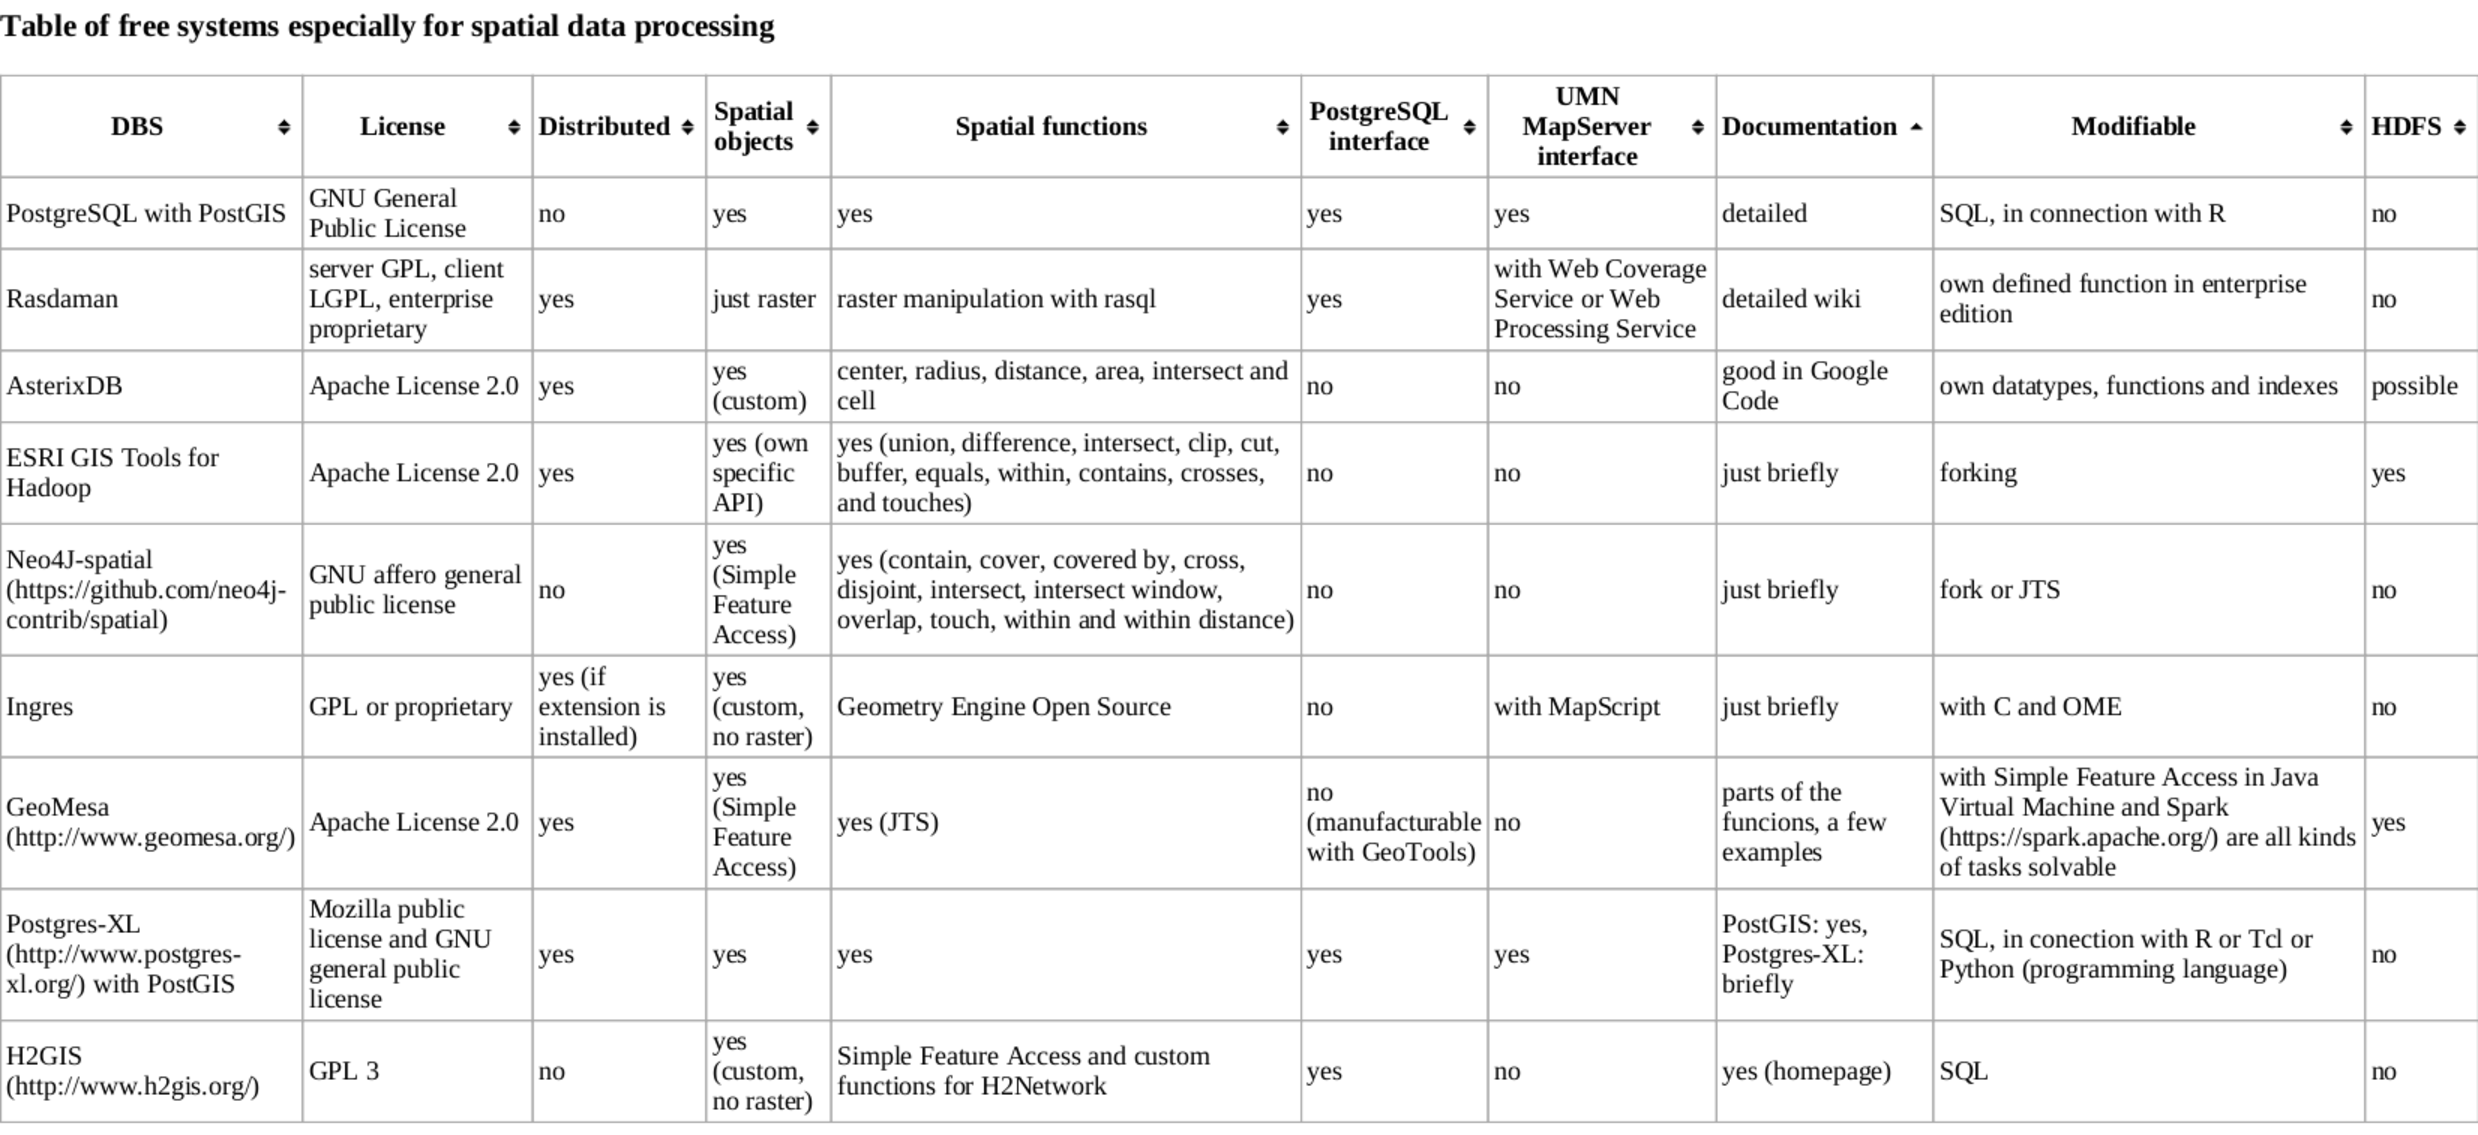
\includegraphics[width=\textwidth]{Abbildungen/table_spatialdatabases.pdf}
\caption[Übersicht relevanter GIS Frameworks]{Übersicht relevanter GIS Frameworks nach \cite{website:wiki-spatialdatabase}}
\label{fig:spatialdatabases}
\end{figure}
Darin sind GIS zur räumlichen Datenverarbeitung mit wesentlichen Eigenschaften wie PostgreSQL Schnittstelle und räumliche Datentypen aufgelistet.
Entsprechend den Anforderungen wurden daraus drei Frameworks für die Nutzwertanalyse ausgewählt.

%TODO: Nutzertanalyse: Struktur, Bewertungssystem, erklären

Tabelle \ref{table:Wertungsmassstab} zeigt die für die Nutzwertanalyse notwendige Wertung der einzelnen Metriken.
\begin{table}[h]
\centering
\begin{tabular}{l|l}
\textbf{Metrik} & \textbf{Gewichtung in \%} \\ \hline
Richtigkeit & 10 \\ \hline
Interoperabilität & 22 \\ \hline
Funktionsumfang & 18 \\ \hline
Fehlertoleranz & 8 \\ \hline
Dokumentation & 20 \\ \hline
Zeitverhalten & 16 \\ \hline
Modifizierbarkeit & 16
\end{tabular}
\caption{Wertungsmaßstab der einzelnen Metriken}
\label{table:Wertungsmassstab}
\end{table}

Für jedes Framework wird eine Nutzwertanalyse durchgeführt und die dazugehörigen Tabellen dazu präsentiert.

Zu jeder Metrik wird der erreichte Wert, die ungewichtete Erfüllung, die gewichtete Erfüllung ein ein Kommentar angegeben.
Die ungewichtete Erfüllung bezieht sich auf den maximal zu erreichenden Wert der Metrik, die gewichtete Erfüllung dagegen auf die Erfüllung der Metrik in Bezug auf \ref{table:Wertungsmassstab}.
Die Kommentarspalte dient der Darstellung des Erreichens der Mindestanforderungen.
Der schlussendliche Nutzwert ergibt sich nach Zangemeister in \cite{website:nutzwertanalyse} aus der Summe der Produkte des Teilnutzens des jeweiligen Kriteriums mit der Gewichtung des Kriteriums.

\section{GeoMesa}

\begin{table}[htp]
\centering
\small
\begin{tabular}{l|c|c|p{3cm}}
%\begin{longtable}[H]{p{35mm}>{\columncolor[gray]{0.97}}p{35mm}}
%\rowcolor[gray]{.9}
\textbf{Metrik} & \textbf{erreichter Wert} & \textbf{Erfüllung in \%} & \textbf{Kommentar} \\ \hline
Funktionsumfang & 44 & 82 & alle Funktionen enthalten \\ \hline
Richtigkeit &  &  &  \\ \hline
Interoperabilität &  &  &  \\ \hline
Fehlertoleranz &  &  &  \\ \hline
Dokumentation &  &  &  \\ \hline
Zeitverhalten &  &  &  \\ \hline
Modifizierbarkeit &  &  &  \\
%\hline \hline
%\textbf{Summe:} &  &  &
\end{tabular}
\caption{Nutzwertanalyse GeoMesa}
\label{table:nutzwertanalyse-geomesa}
\end{table}
%\end{longtable}



\section{ESRI GIS Tools for Hadoop}

